\chapter{Исследовательский раздел}

В рамках данной работы было решено провести два исследования. Предметом исследований является поисковый запрос, а именно кеширование его результатов. Перед обращением к базе данных, сначала проверяется кеш, если ли в нем результат данного поискового запроса. Если есть, то запрос в базу данных не осуществляется, а пользователю возвращаются закешированные данные. 

Данные о производительности измерялись на основе множественного запуска запросов поиска на десяти случайно выбранных заранее поисковых строках одинаковой длины. Для всех вариантов кеширования и сериализации в рамках одного тестирования, набор поисковых строк одинаков.

Характеристики устройства, на котором проводилось исследование, следующие~\cite{macbook}:

\begin{itemize}
	\item оперативная память 8Гб;
	\item процессор Apple M2;
	\item операционная система macOS Ventura 13.0.
\end{itemize}

\section{Исследование скорости работы поиска с кешированием и без}
В рамках данного исследования проводилось сравнение скорости работы поиска без использования кеша и с использованием кеша двух видов: Redis~\cite{redis} и кеша в оперативной памяти. Результаты замеров времени работы поиска от количества сотрудников, отделов и команд, которых, в рамках данного исследования, одинаковое количество, представлены в таблице \ref{table:research1}

\begin{table}[h!]
\caption{Зависимость времени выполнения запроса от количества записей с кешированием и без}
\label{table:research1}
\begin{tabular}{|r|r|r|r|l}
\cline{1-4}
\multicolumn{1}{|l|}{\begin{tabular}[c]{@{}l@{}}Количество \\ записей\end{tabular}} & \multicolumn{1}{l|}{\begin{tabular}[c]{@{}l@{}}Время \\ без кеша, мкс\end{tabular}} & \multicolumn{1}{l|}{\begin{tabular}[c]{@{}l@{}}Время \\ с кешем в Redis, мкс\end{tabular}} & \multicolumn{1}{l|}{\begin{tabular}[c]{@{}l@{}}Время \\ с кешем в ОЗУ, мкс\end{tabular}} &  \\ \cline{1-4}
5000                                                                                & 48099                                                                               & 1855                                                                                       & 175                                                                                                        &  \\ \cline{1-4}
10000                                                                               & 47488                                                                               & 2286                                                                                       & 686                                                                                                        &  \\ \cline{1-4}
15000                                                                               & 64490                                                                               & 3455                                                                                       & 693                                                                                                        &  \\ \cline{1-4}
20000                                                                               & 72954                                                                               & 4173                                                                                       & 706                                                                                                        &  \\ \cline{1-4}
25000                                                                               & 196815                                                                              & 4132                                                                                       & 1047                                                                                                       &  \\ \cline{1-4}
30000                                                                               & 200044                                                                              & 4290                                                                                       & 1236                                                                                                       &  \\ \cline{1-4}
\end{tabular}
\end{table}

\newpage

Результаты замеров также представлены в графическом формате на рисунке~\ref{img:research1}.

\begin{figure}[h!]
\centering
    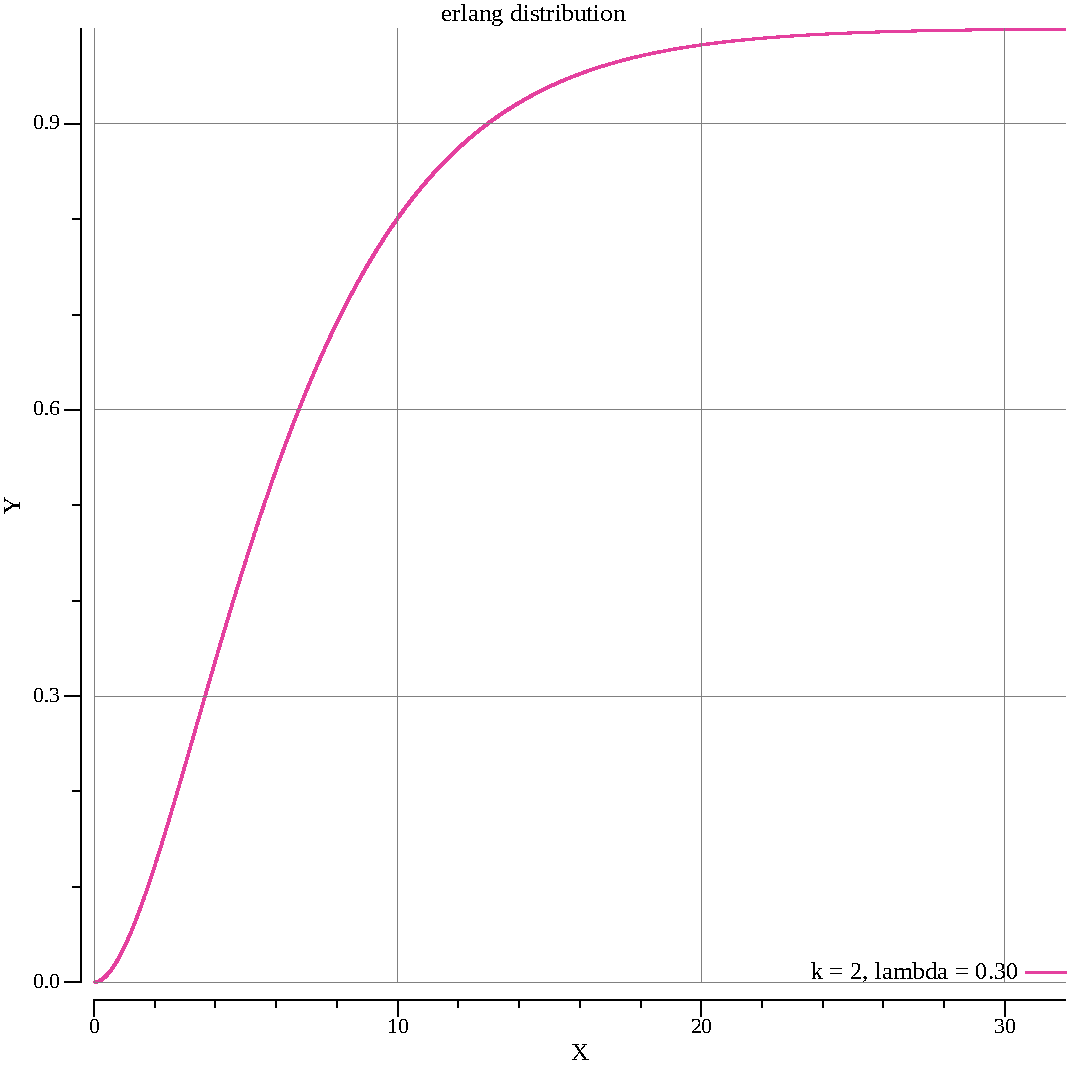
\includegraphics[width=0.7\linewidth]{assets/1.pdf}
    \caption{Зависимость времени выполнения запроса от количества записей с кешированием и без}
    \label{img:research1}	
\end{figure}

Исследуемая функция работает быстрее с кешированием. При этом, кеширование в оперативной памяти работает быстрее, чем кеширование в Redis на заданной выборке. Это связано в том числе с тем, что при использовании кеша в оперативной памяти, отсутствуют сетевые задержки при получении и отправке данных~\cite{redis}.

При объеме данных в 30 тысяч записей, запрос с использованием кеша в Redis работает примерно в 46 раз быстрее, чем без кеша. При этом, запрос с использованием кеша в оперативной памяти, работает быстрее реализации с кешем в Redis примерно в 3.4 раза.

\section{Исследование скорости работы поиска с использованием различных методов сериализации при использовании кеширования в Redis}

В рамках данного исследования проводилось сравнение скорости работы функции поиска с использованием различных алгоритмов сериализации при кешировании в Redis. В отличие от кеша в оперативной памяти, Redis хранит данные, в данном случае, в строковом формате, поэтому для хранения структуры необходимо сериализовать ее, затем преобразованную строку помещать в кеш.

В данном случае сравниваются популярные форматы сериализации JSON~\cite{json} и CBOR~\cite{cbor}. Кроме того, исследуется комбинация заданных форматов с алгоритмом сжатия Gzip~\cite{gzip}. Для реализации методов сериализации используются соответствующие библиотеки~\cite{json_doc, cbor_doc, gzip_doc}. Результаты замеров времени для различных вариантов сериализации в зависимости от объема хранимых данных представлены в таблице \ref{table:research2} и на рисунке \ref{img:research2}.

\newpage

\begin{table}[h!]
\caption{Зависимость времени выполнения запроса от количества записей для разных методов сериализации}
\label{table:research2}	
\begin{tabular}{|r|r|r|r|r|l}
\cline{1-5}
\multicolumn{1}{|l|}{\begin{tabular}[c]{@{}l@{}}Количество \\ записей\end{tabular}} & \multicolumn{1}{l|}{JSON, мкс} & \multicolumn{1}{l|}{CBOR, мкс} & \multicolumn{1}{l|}{JSON+Gzip, мкс} & CBOR+Gzip, мкс &  \\ \cline{1-5}
5000                                                                                & 1447                           & 1049                           & 1208                                & 1111           &  \\ \cline{1-5}
10000                                                                               & 2098                           & 1527                           & 1777                                & 1467           &  \\ \cline{1-5}
15000                                                                               & 2487                           & 1802                           & 3056                                & 1879           &  \\ \cline{1-5}
20000                                                                               & 3518                           & 2297                           & 3393                                & 2402           &  \\ \cline{1-5}
25000                                                                               & 3861                           & 2814                           & 3634                                & 2972           &  \\ \cline{1-5}
30000                                                                               & 4373                           & 3595                           & 3458                                & 3267           &  \\ \cline{1-5}
\end{tabular}
\end{table}

\begin{figure}[h!]
\centering
    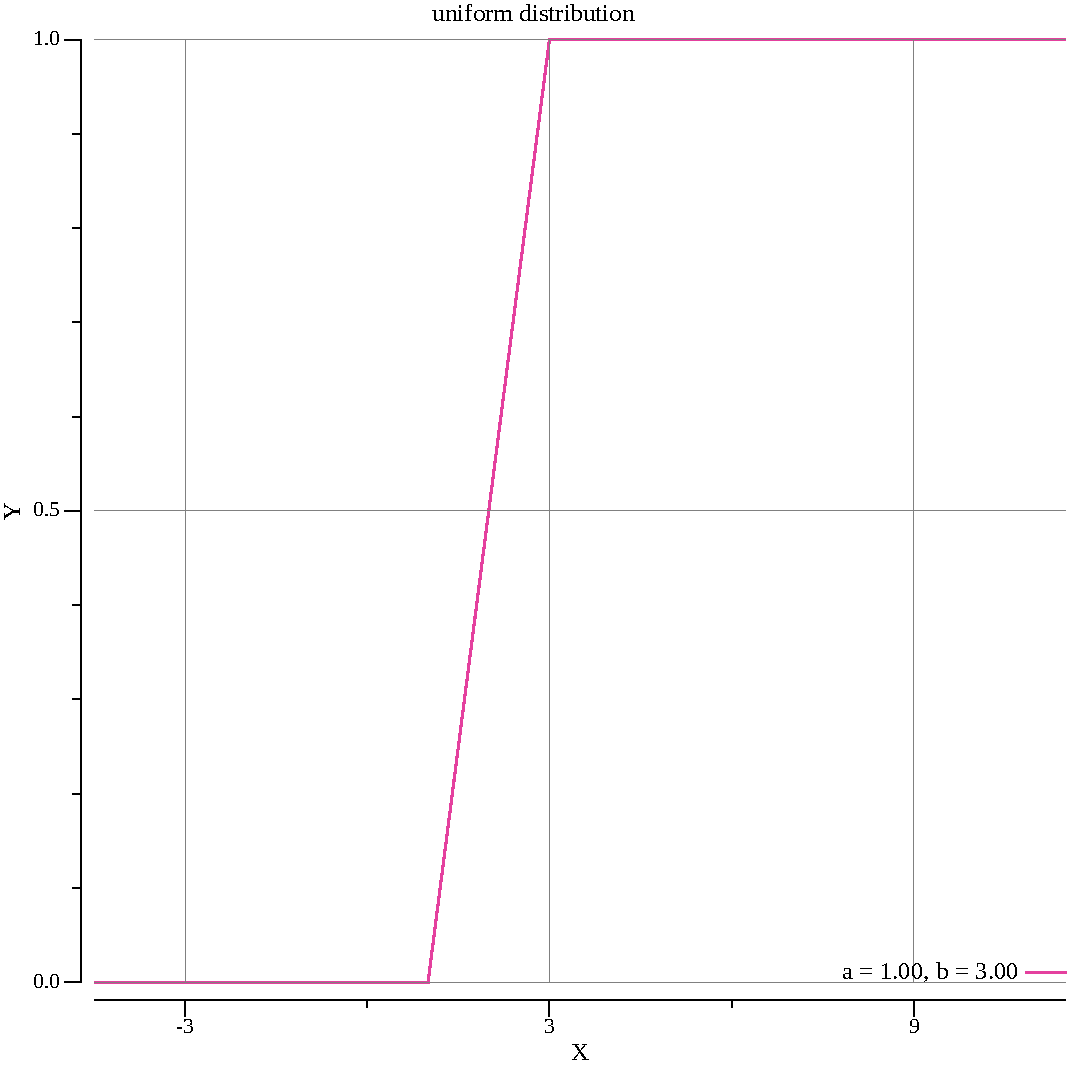
\includegraphics[width=0.7\linewidth]{assets/2.pdf}
    \caption{Зависимость времени выполнения запроса от количества записей для разных методов сериализации}
    \label{img:research2}	
\end{figure}

При объеме данных в 30 тысяч записей, самым долгим методом является сериализация в JSON, самым быстрым~---~сериализация в CBOR с использованием алгоритма сжатия Gzip. Разница во времени работы составляет примерно 1.3 раза. При этом, реализация с использованием комбинации JSON и Gzip работает также быстрее реализации JSON без архивации, несмотря на большее количество операций. Такое поведение может быть связано с тем, что заархивированные данные занимают меньше места и быстрее передаются по сети.

\section{Исследование объема занимаемой закешированными данными памяти при использовании различных алгоритмов сериализации}

В рамках данного исследование производились замеры суммарного объема занимаемой ключами в Redis памяти в зависимости от количества записей в базе данных. Результаты замеров представлены в таблице \ref{table:research3} и на рисунке \ref{img:research3}.

\begin{table}[h!]
\caption{Зависимость объема занимаемой памяти от количества записей для разных методов сериализации}
\label{table:research3}	
\begin{tabular}{|r|r|r|r|r|l}
\cline{1-5}
\multicolumn{1}{|l|}{\begin{tabular}[c]{@{}l@{}}Количество \\ записей\end{tabular}} & \multicolumn{1}{l|}{JSON, Б} & \multicolumn{1}{l|}{CBOR, Б} & \multicolumn{1}{l|}{JSON+Gzip, Б} & CBOR+Gzip, Б &  \\ \cline{1-5}
5000                                                                                & 172880                       & 111920                       & 35104                             & 30176        &  \\ \cline{1-5}
10000                                                                               & 297088                       & 191856                       & 56928                             & 48544        &  \\ \cline{1-5}
15000                                                                               & 432624                       & 276576                       & 80576                             & 68512        &  \\ \cline{1-5}
20000                                                                               & 562256                       & 365536                       & 103440                            & 87760        &  \\ \cline{1-5}
25000                                                                               & 762032                       & 490624                       & 138416                            & 117504       &  \\ \cline{1-5}
30000                                                                               & 898544                       & 577760                       & 162192                            & 137536       &  \\ \cline{1-5}
\end{tabular}
\end{table}

\begin{figure}[h!]
\centering
    \includegraphics[width=0.7\linewidth]{assets/2_memory.pdf}
    \caption{Зависимость объема занимаемой памяти от количества записей для разных методов сериализации}
    \label{img:research3}	
\end{figure}

При объеме данных в 30 тысяч записей, самым эффективным в плане потребляемой памяти является метод сериализации CBOR в комбинации с алгоритмом сжатия Gzip. Использование сжатия позволяет сократить потребление памяти примерно в 5.5 раз для JSON и примерно в 3.2 раза для CBOR. Такое значительное сокращение объема данных позволяет ускорить получение данных из кеша из-за меньшего объема данных, передаваемого по сети, что и показано в предыдущем исследовании.


